%
\chapter{Metodologia}
\label{chap:metodologia}

\section{Descrição do Processo} \label{sec:descricaoprocesso}

Como já mencionado no \autoref{chap:introducao}, o processo modelado
neste trabalho utilizou os dados publicados por \citeonline{Rojas2014a}. 

\subsection{Diagrama Esquemático} \label{sec:diagramaesquematico}

O reator é composto de dois leitos catalíticos, carregados de forma densa
(\emph{dense loading}). No topo de ambos os leitos há catalisador carregado de
forma solta (\emph{sock loading}). A carga é composta de gasolina de pirólise,
hidrogênio e parte do produto hidrogenado reciclado. Este último é parte da
corrente líquida oriunda de um vaso de separação, cuja carga é a corrente de
saída do reator. Parte da corrente líquida do vaso de separação também
funciona como corrente de resfriamento, que é injetada entre os dois leitos
catalíticos para controle de temperatura (\emph{quench}). Um diagrama
simplificado que ilustra o reator está na \autoref{fig:esquemareator}. 

\begin{figure}[htb]
\centering 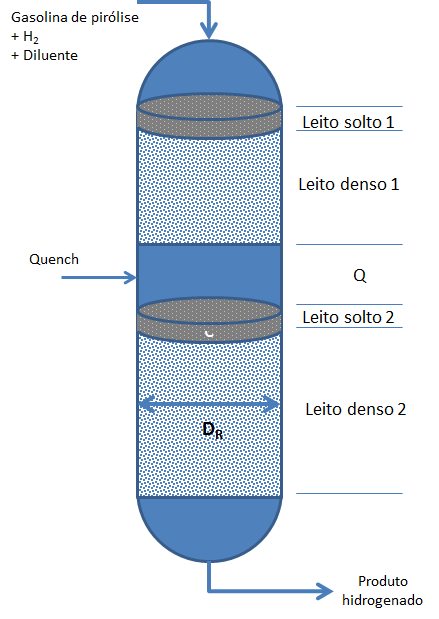
\includegraphics[scale=0.75]{images/Chap3/esquemareator.png}
\caption{Diagrama esquemático do reator \cite{Rojas2014a}.}
\label{fig:esquemareator}
\end{figure}

A \autoref{tab:dadosreator} apresenta as dimensões do reator.

\begin{table}[!htb]
\begin{center}
\caption{Dados do Reator \cite{Rojas2014a}.}
\label{tab:dadosreator}
\small
\begin{tabular}{lcc}
{Dimensão} & {Variável} & {Valor}
\\
\hline
{Diâmetro do Reator} & {$D_R$} & $3,047$ m \\
{Comprimento do Leito Solto 1} & {$L_{sl1}$} & $0,13$ m \\
{Comprimento do Leito Denso 1} & {$L_{dl1}$} & $2,97$ m \\
{Comprimento do Leito Solto 2} & {$L_{sl2}$} & $0,38$ m \\
{Comprimento Leito Denso 2} & {$L_{dl2}$} & $2,97$ m \\
{Zona de Quench} & {$L_{Q}$} & $1,55$ m \\
\bottomrule
\end{tabular}
\end{center}
\end{table}

\nomenclature{$L_{sl1}$}{Comprimento do leito solto 1 \nomunit{m}}
\nomenclature{$L_{dl1}$}{Comprimento do leito denso 1 \nomunit{m}}
\nomenclature{$L_{sl2}$}{Comprimento do leito solto 2 \nomunit{m}}
\nomenclature{$L_{dl2}$}{Comprimento do leito denso 2 \nomunit{m}}
\nomenclature{$L_{Q}$}{Comprimento da zona de quench \nomunit{m}}

\subsection{Catalisador} \label{sec:catalisador}

O catalisador considerado na modelagem contém Pd suportado em alumina
($Al_2O_3$), de formato esférico. Além desses dados, foi fornecida a informação
de volume total de poros $Vt_{poros}$ = $5,5.10^{-4}$ $m^3/kg$. O dado de volume
total de poros não é suficiente por si só para calcular a porosidade dos leitos,
como é apresentado na \autoref{sec:propriedadesleitoscataliticos}. Assim,
adotou-se a massa específica do $Al_2O_3$ puro ($\rho_{Al_2O_3}$ = $3940$
$kg/m^3$) para a massa específica da parte sólida das partículas de catalisador.

\nomenclature{$Vt_{poros}$}{Volume total de poros \nomunit{m^3/kg}}
\nomenclature[G]{$\rho_{Al_2O_3}$}{Massa específica do óxido de alumínio
\nomunit{kg/m^3}}

\subsection{Porosidade dos Leitos Catalíticos}
\label{sec:propriedadesleitoscataliticos}

Antes de determinar a porosidade dos leitos catalíticos, é preciso avaliar a
massa específica das partículas ($\rho_{p}$). Este parâmetro, calculado pela
\autoref{eq:rhoparticula}, é estimado em $1244 kg/m^3$.

\begin{equation}
\rho_{p} = \dfrac{1}{Vt_{poros}+\dfrac{1}{\rho_{Al_2O_3}}}
\label{eq:rhoparticula}
\end{equation}

\nomenclature[G]{$\rho_{p}$}{Massa específica da partícula de catalisador
\nomunit{kg/m^3}}

A porosidade de cada um dos leitos pode ser calculada, portanto, pela
\autoref{eq:porosidade}, como segue:

\begin{equation}
\epsilon_{B} = \dfrac{V_{l}-\dfrac{\rho_{B}V_l}{\rho_{Al_2O_3}}}{V_l}
\label{eq:porosidade}
\end{equation}

sendo $V_l$ o volume do leito e $\rho_B$ a
massa específica de um leito catalítico logo após o seu carregamento. 

Utilizando os dados apresentados na \autoref{sec:catalisador}, e utilizando os
valores de massa específica \emph{bulk} dos leitos $\rho_{B}$ publicados por
\citeonline{Rojas2014a}, chega-se nos valores mostrados na
\autoref{tab:dadosdosleitos}.

\begin{table}[!htb]
\begin{center}
\caption{Dados dos Leitos Catalíticos \cite{Rojas2014a}.}
\label{tab:dadosdosleitos}
\small
\begin{tabular}{ccc}
{ - } & {Densidade \emph{bulk} ($kg/m^3$)} & {Porosidade} 
\\
\hline
{Leito 1} & $814$ & $0,346$ \\
{Leito 2} & $813$ & $0,347$ \\
\bottomrule
\end{tabular}
\end{center}
\end{table}

\subsection{Composição das Correntes} \label{sec:composicaocorrentes}

A composição das correntes de entrada e de quench estão na
\autoref{tab:composicao}. Para o presente trabalho, utilizou-se
apenas os valores da primeira corrida publicados por
\citeonline{Rojas2014a}, já que para este caso foram publicados
também dados industriais.

As propriedades termodinâmicas dos compostos $28$ e $29$ não foram
encontradas. Assim, eles foram considerados como sendo parte dos compostos
$26$ e $27$, respectivamente.

\begin{table}[!htb]
\begin{center}
\caption{Composição das correntes de entrada e de quench \cite{Rojas2014a}.}
\label{tab:composicao}
\small
\begin{tabular}{clcc}
{Identificador $i$} & {Composto} & Entrada (\% mássica) & Quench (\% mássica)
\\
\hline
1 & Hidrogênio				& $0,48$ & $0,08$ \\
2 & Metano					& $0,52$ & $0,70$ \\
3 & Etano					& $0,12$ & $0,11$ \\
4 & n-Propano				& $0,36$ & $0,27$ \\
5 & n-Butano				& $0,30$ & $0,24$ \\
6 & n-Pentano				& $5,40$ & $5,60$ \\
7 & trans-2-Penteno			& $5,30$ & $7,60$\\
8 & trans-1,3-Pentadieno	& $2,50$ & $0,23$ \\
9 & Ciclopentano			& $1,50$ & $2,60$ \\
10& Ciclopenteno			& $2,10$ & $3,00$ \\
11& Metil-1,3-Ciclopentadieno	& $1,90$ & $0,21$ \\
12& n-Hexano				& $3,30$ & $3,30$ \\
13& Metilciclopentano		& $1,60$ & $1,70$ \\
14& Metilciclopenteno		& $2,00$ & $2,60$ \\
15& 1,3-Ciclopentadieno		& $1,90$ & $0,02$ \\
16& Benzeno					& $28,90$ & $30,10$ \\
17& n-Heptano				& $2,80$ & $2,90$ \\
18& Tolueno					& $16,00$ & $16,30$ \\
19& n-Octano				& $1,30$ & $1,30$ \\
20& Etilbenzeno				& $3,40$ & $5,40$ \\
21& Estireno				& $2,00$ & $0,11$ \\
22& Xileno					& $5,40$ & $5,50$ \\
23& n-Nonano				& $0,66$ & $0,72$ \\
24& 1-Metil-3-Etilbenzeno	& $2,90$ & $3,90$ \\
25& Metilestireno			& $1,40$ & $0,31$ \\
26& Dihidrodiciclopentadieno	& $1,80$ & $3,00$ \\
27& Diciclopentadieno		& $1,80$ & $0,12$ \\
28& Metildihidrodiciclopentadieno	& $1,50$ & $2,20$ \\
29& Metildiciclopentadieno	& $0,88$ & $0,11$ \\
\bottomrule
\end{tabular}
\end{center}
Onde $i$ é o número identificador do composto na simulação a ser apresentada.
\end{table}

\nomenclature[S]{$i$}{i-ésimo componente}

\subsection{Condições de operação} \label{sec:condicaocomposicaocorrentes}

As condições de operação consideradas inicialmente estão na
\autoref{tab:condicoesoperacao}. No \autoref{chap:resultados} há uma discussão
sobre a validade de algumas dessas variáveis aqui apresentadas.

\begin{table}[!htb]
\begin{center}
\caption{Dados do Reator \cite{Rojas2014a}.}
\label{tab:condicoesoperacao}
\small
\begin{tabular}{lcc}
{Dimensão} & {Variável Discretizada} & {Valor}
\\
\hline
{Pressão de entrada} & {$P_{1}$} & $5,03$ MPa \\
{Temperatura de entrada} & {$T_{1}$} & $366,15$ K \\
{Vazão mássica de entrada} & {$F_{w,1}$} & $2,477.10^5$ kg/h \\
{Pressão da corrente de \emph{quench}} & {$P_{Q}$} & $4.6$ MPa \\
{Temperatura da corrente de \emph{quench}} & {$T_{Q}$} & $326,15$ K \\
{Vazão mássica da corrente de quench} & {$F_{w,Q}$} & $2,079.10^4$ kg/h \\
\bottomrule
\end{tabular}
\end{center}
\end{table}

\section{Premissas} \label{sec:premissas}

\subsection{Premissas adotadas por \citeonline{Rojas2014a}}
\label{sec:premissasrojas}

Antes de apresentar as premissas que nortearam o presente trabalho, vale
aqui apresentar, para efeito de comparação, as premissas utilizadas por
\citeonline{Rojas2014a}.

\begin{enumerate}
  \item O reator opera em estado estacionário e adiabaticamente.
  \item Gradientes radiais são desprezíveis.
  \item Dispersões axiais foram negligenciadas; portanto, assumiu-se o
  escoamento empistonado para ambas as fases líquida e gasosa.
  \item A fase gasosa está em excesso; dessa forma, negligenciou-se a
  resistência a transferência de massa na fase gasosa.
  \item Fator de molhamento, atividade catalítica e densidade do leito
  uniformes.
  \item A transferência de calor entre as fases e no interior das partículas de
  catalisador foram desprezadas.
  \item A entalpia de dissolução de compostos na fase gás, bem como calor de
  vaposização de líquido foram desprezadas.
  \item A região do quench é assumida como sendo um tambor \emph{flash}, que atinge o
  equilíbrio instantaneamente.
  \item A corrente de saída do primeiro leito mistura-se instantaneamente com a
  corrente de quench.
  \item O reator opera em regime de borbulhamento.
  \item Reações reversíveis e isomerizações foram negligenciadas.
  \item As reações ocorrem somente na interface líquido-sólido.
  \item A desativação catalítica foi desprezada.
\end{enumerate}

No presente estudo, algumas premissas adotadas por \citeonline{Rojas2014a} serão
alteradas, como será descrito a seguir. 

\subsection{Premissas deste trabalho} \label{sec:premissasdestetrabalho}

Como já mencionado no \autoref{chap:introducao}, um dos objetivos do presente
trabalho é avaliar algumas respostas dinâmicas ao processo proposto. Além disso,
a implementação da modelagem foi feita em \emso, software que avalia respostas
dinâmicas por concepção. Assim, convenientemente, a premissa de um reator
operando em estado estacionário foi descartada. Permanece, porém, aqui, a
premissa de que o equipamento opere de forma adiabática.

A alteração mais importante às premissas adotadas por \citeonline{Rojas2014a}, e
que representa um avaço por eles publicado, é a consideração tanto da entalpia
de dissolução do hidrogênio na fase líquida quanto da entalpida de vaporização
de líquido. Isso foi possível graças à abordagem de modelagem por células,
assunto da seção \autoref{sec:modelagemredecelulas}.

Portanto, ficam aqui definidas as seguintes premissas:

\begin{enumerate}
  \item O reator opera adiabaticamente.
  \item Gradientes radiais são desprezíveis.
  \item Dispersões axiais foram negligenciadas; portanto, assumiu-se o
  escoamento empistonado para ambas as fases líquida e gasosa.
  \item A fase gasosa está em excesso; dessa forma, negligenciou-se a
  resistência a transferência de massa na fase gasosa.
  \item Fator de molhamento, atividade catalítica e densidade do leito
  uniformes.
  \item A transferência de calor entre as fases e no interior das partículas de
  catalisador foram desprezadas.
  \item A região do \emph{quench} é assumida como sendo um tambor \emph{flash}, que
  atinge o equilíbrio instantaneamente.
  \item A corrente de saída do primeiro leito mistura-se instantaneamente com a
  corrente de \emph{quench}.
  \item O reator opera em regime de borbulhamento.
  \item Reações reversíveis e isomerizações foram negligenciadas.
  \item As reações ocorrem somente na interface líquido-sólido.
  \item A desativação catalítica foi desprezada.
\end{enumerate}

Um dos motivos de se manter praticamente inalteradas as premissas adotadas por
\citeonline{Rojas2014a} foi o de realiar comparações entre os dois estudos.

Negligenciar os gradientes e dispersões de calor e massa, tanto radialmente
quanto axialmente, é uma recomendação muito comum encontrada na literatura
\cite{Ancheyta2011, Ranade2011, Froment2011} para simulações cujo objetivo é
prever o comportamento de um TBR, sob o ponto de vista de liberação de calor e
conversão das reações. Da mesma forma é a desconsideração da transferência de
calor entre as fases.

Como já mencionado no \autoref{chap:revisaobibliografica},
\citeonline{Rojas2014a} utilizaram as reações publicadas por
\citeonline{Hanika1999}. Isso pode ter motivado os autores a negligenciar a
resistencia à transferência de massa na fase gasosa.

As premissas assumidas para a região de \emph{quench} são bastante razoáveis, já
que normalmente os projetistas de reatores TBR desejam a corrente oriunda do
leito superior se misture rapidamente com a corrente de \emph{quench},
homogeneizando a carga para o segundo leito. Uma mistura inadequada entre as
correntes de entrada na região de \emph{quench} pode levar a caminhos
preferenciais e regiões de estagnação no leito inferior \cite{Ancheyta2011}.

O regime de operação por borbulhamento foi adotado para que as
equações hidrodinâmicas fossem as mesmas utilizadas por \citeonline{Rojas2014a}.
Contudo, uma verificação da validade dessa premissa é apresentada no
\autoref{chap:resultados}.

\section{Modelagem por Rede de Células} \label{sec:modelagemredecelulas}

Para utilizar a abordagem de modelagem por rede de células, cada leito
catalítico foi subdivido em células em seu comprimento, i.e., discretizado em
$N_{Disc}$ segumentos de leito. Cada seguimento de leito fica identificado por
um índice ($z$). A figura \autoref{fig:celula} ilustra uma célula de leito de
reator. Do ponto de vista reacional, cada célula representará um reator CSTR
associado a um tambor de \emph{flash}. Nesse tambor de \emph{flash}, mantém-se a premissa
de que o equilíbrio termodinâmico é atingido instantaneamente.

 \begin{figure}[htb]
 \centering 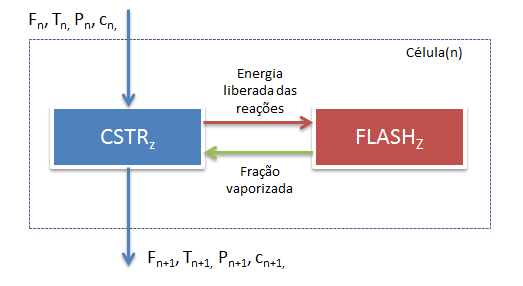
\includegraphics[scale=0.75]{images/Chap3/celula.png}
 \caption{Elemento discretizado de leito - célula}
 \label{fig:celula}
 \end{figure}

\nomenclature{$N_{Disc}$}{Número de células de um leito do reator}
\nomenclature[S]{$z$}{z-ésima célula de leito de reator}

Para a região de quench, será usado um tambor de \emph{flash}, onde o equilíbrio
termodinâmico é também atingido instantaneamente. A \autoref{fig:quench} ilustra
a região de quench.

 \begin{figure}[htb]
 \centering 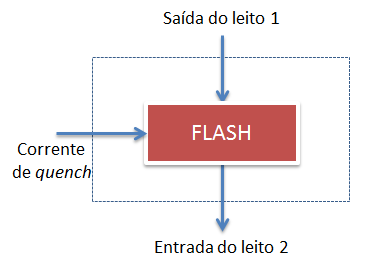
\includegraphics[scale=0.75]{images/Chap3/quench.png}
 \caption{Região de quench do reator}
 \label{fig:quench}
 \end{figure}

Com esse tipo de abordagem, foi possível considerar os efeitos termodinâmicos
ao longo do reator, como também prever a composição das fases líquida e
gasosa. As próximas seções apresentam o equacionamento construído

\section{Balanço de Massa e Energia} \label{sec:balancomassaenergia}

Normalmente, para a modelagem de TBR heterogênea, os autores que utilizam
modelos determinísticos contínuos fazem o balanço de massa para todas as
fases separadamente, i.e., para cada fase é feito o balanço de massa por
componente. %\citeonline{Ancheyta2011} apresenta de uma forma didática as
% equações de balanço de massa de cada fase, considerando e explicando todos os
% efeitos (dispersões, reações, transferências de massa).
Cada pesquisador, portanto, de acordo com a premissa adotada, elimina muitos dos
termos das equações de balanço, a fim simplificar o modelo e facilitar a
solução. 

Para este trabalho, diante das premissas adotadas, a equação de balanço de massa
está mostrada na \autoref{eq:balancodemassa}. Nessa equação, foi considerado o
termo de diferenciação da massa $M$ de cada componente $i$, em cada célula $z$,
no tempo $t$. Dessa forma, é possível o estudo de respostas dinâmicas do
processo.

\begin{equation}
\dfrac{dM_{i,z}}{dt} = F_zC_{i,z} - F_{z+1}C_{i,z+1} +
\displaystyle\sum_{j=1}^{N_{reac}} \nu_{i,j}r_{j,z} \dfrac{W}{N_{Disc}}
\label{eq:balancodemassa}
\end{equation}

onde $M_{i,z}$ é a massa do componente $i$ na célula $z$, $j$ é o número
identificador de cada reação, $N_{reac}$ é o número total de reações,
$\nu_{i,j}$ é o coeficiente do componente $i$ na reação $j$, $r_{j,z}$ é taxa
da reação $j$ na célula $z$, $F$ é a vazão molar total e $W$ é a massa total de
catalisador presente no leito.

\nomenclature{$M$}{Massa \nomunit{kmol}}
\nomenclature{$N_{reac}$}{Número total de reações}
\nomenclature{$r$}{Taxa de reação \nomunit{kmol/(kg_{cat}.h)}}
\nomenclature{$F$}{Vazão molar \nomunit{kmol/h}}
\nomenclature{$W$}{Massa total de catalisador em um leito\nomunit{kg}}
\nomenclature[S]{$j$}{j-ésima reação}
\nomenclature[G]{$\nu$}{Coeficiente de reação}

A \autoref{eq:balancodeenergia} mostra o balanço de energia de forma
discretizada.

\begin{equation}
\dfrac{dE_{z}}{dt} = F_zh_{z} - F_{z+1}h_{z+1} +
\displaystyle\sum_{j=1}^{N_{reac}} \Delta H_{j}r_{j,z} \dfrac{W}{N_{Disc}}
\label{eq:balancodeenergia}
\end{equation}

onde $E_{z}$ é a energia na célula $z$,  $h$ é a entalpia da
corrente $F$ e $\Delta H_{j}$ o calor envolvido na reação $j$.

\nomenclature{$E$}{Energia \nomunit{kJ}}
\nomenclature{$h$}{Entalpia \nomunit{kJ/kmol}}
\nomenclature[G]{$\Delta H$}{Calor de reação \nomunit{kJ/kmol}}

As \autoref{eq:balancodemassa} e \autoref{eq:balancodeenergia}, somadas a
corrente $F$ e seu cálculo de ELV, permitem determinar a fração vaporizada,
composição das fases e respectivas propriedades físicas em cada célula $z$.

É importante notar ainda que, da forma como as \autoref{eq:balancodemassa} e
\autoref{eq:balancodeenergia} estão escritas, massa e energia contidas em cada
célula são grandezas extensivas. 

\section{Cinética das Reações} \label{sec:cineticadasreacoes}

As reações de hidrogenação e os parâmetros cinéticos estão na
\autoref{tab:composicao}. Conforme já explicado, o sistema reacional foi
considerado como sendo um conjunto de hidrogenações irreversíveis e
independentes da concentração de hidrogênio. A constante de pseudo-primeira
ordem da reação $j$ na célula $z$, $k^{'}_{j,z}$, está definido na
\autoref{eq:constantepseudoprimeiraordem}.

\begin{equation}
k^{'}_{j,z} = \eta_ik_jC^{*}_{H_2}
\label{eq:constantepseudoprimeiraordem}
\end{equation}

sendo $\eta$ o fator de efetividade de intradifusão, $k$ a
constante de taxa de reação instrínseca e $C^{*}_{H_2}$ a concentração de
equilíbrio de hidrogênio em fase líquida.

\nomenclature{$k^{'}$}{Constante de taxa de reação de pseudo-primeira
ordem \nomunit{kg/(kg_{cat}.h)}}
\nomenclature{$k$}{Constante de taxa de reação intrínseca
\nomunit{kg.m^3/(kg_{cat}.h.kmol_{H_2})}}
\nomenclature{$C^{*}_{H_2}$}{Concentração de equilíbrio de hidrogênio em fase
líquida \nomunit{kmol/m^3} \nomunit{kJ/kmol}}
\nomenclature[G]{$\eta$}{Fator de efetividade de intradifusão}

Portanto, a taxa $r$ da reação $j$ na célula $z$ será dada pela
\autoref{eq:taxareacao}:

\begin{equation}
r_{j,z} = k^{*}_{j,z}C^{S}_{i,z}
\label{eq:taxareacao}
\end{equation}

onde o vetor $C^{S}$ representa a concentração das espécies químicas na fase
sólida. Essa concentração é determinada pela transferência de massa
líquido-sólido, como está apresentado na \autoref{sec:interfaceliquidosolido}.

A constante da taxa de reação específica $k^{*}$ é calculada pela
equação de van't Hoff, na $T^{ref}$ = $417 K$, como segue:

\begin{equation}
k^{*}_{j,z} = \dfrac{k^{'}_{j,z}} {\rho^{L}_{z+1}} \exp
\left[{\dfrac{-Ea_j}{R} \left (\dfrac{1}{T_{z+1}} -
\dfrac{1}{T^{ref}} \right )}\right]
\label{eq:constantetaxareacaoespecifica}
\end{equation}

sendo $\rho^L$ a massa específica da fase líquida.

Nota-se na equação \autoref{eq:constantetaxareacaoespecifica} que foram usadas
temperatura e massa específica da corrente de saída da célula ($z+1$). Essa
opção foi feita de forma abritrária, já que poderiam ser usadas as condições de
entrada da mesma forma.

\nomenclature{$k^{*}$}{constante da taxa de reação específica
\nomunit{kmol/(m^3/(kg_{cat}.h)}}
\nomenclature[R]{$L$}{Designação da fase líquida}
\nomenclature[R]{$S$}{Designação da fase sólida}
\nomenclature{$T^{ref}$}{Temperatura de referência, $417 K$}
\nomenclature[G]{$\rho$}{Massa específica \nomunit{kg/m^3}}
\nomenclature{$T$}{Temperatura \nomunit{K}}
\nomenclature{$R$}{Constante universal dos gases ideais \nomunit{kJ/(kmol.K)}}
\nomenclature{$Ea$}{Energia de ativação \nomunit{kJ/kmol}}
\nomenclature[S]{$B$}{Leito catalítico}
\nomenclature{$C$}{Concentração \nomunit{kmol/m^3}}

\section{Termodinâmica} \label{sec:termodinamica}

A abordagem termodinâmica utilizada para prever o ELV foi a $\phi_i$ -
$\phi_i$, a mesma utilizada por \citeonline{Rojas2014a}, com a EoS de SRK
\cite{Soave1972}, e seguindo as recomendações e os parâmetros do trabalho feito
por \citeonline{Zhou2006} para a solubilidade de hidrogênio em gasolina de
pirólise. Esta recomendação consiste em utilizar a regra de mistura clássica de
van der Waals \cite{VanderWaals1873}, com parâmetros de interação binária
específicos para cada um dos pares de hidrogênio/hidrocarboneto. Para o caso da
regra de mistura escolhida, os parâmetros cruzados $aij$ estão definidos pela
\autoref{eq:parametroaij} \cite{Peng1976,Soave1972}.

\begin{equation}
a_{i,j} = \sqrt{a_ia_j}(1-\delta_{ij})
\label{eq:parametroaij}
\end{equation}

Para a avaliação do ELV e demais propriedades, foi utilizado o pacote
termodinâmico do simulador de processos iiSE (\emph{Industrial Integrated
Simulation Environment}). Para tanto, foi criada uma simulação no iiSE, onde
foram colocadas as composições da carga e da corrente de quench. O \emso, por
sua vez, utiliza a simulação criada em iiSE para os cálculos termodinâmicos, e
somente para este fim. 

Para finalizar esta seção, vale esclarecer que, da forma como foi implementada
no \emso, a corrente $F$ não só contém a informação de vazão e composição molar
(total e por componente), mas tabém possui uma rotina de cálculo de
\emph{flash}, utilizando como variáveis de entrada pressão, temperatura e
composição global. Dessa forma, ficam incluídos os efeitos de dissolução de
hidrogênio na fase líquida bem como a vaporização da fase líquida.

\nomenclature[G]{$\phi$}{Coeficiente de fugacidade}
\nomenclature[G]{$\delta_{ij}$}{Parâmetro de interação binária}
\nomenclature[Z]{iiSE}{\emph{Industrial Integrated Simulation Environment}}
\nomenclature{$a_{ij}$}{Parâmetro cruzado entre as espécies $i$ e $j$}
\nomenclature{$a$}{Parâmetro de atração}

\section{Interface Líquido-Sólido} \label{sec:interfaceliquidosolido}

Como a transferência de massa gás-líquido foi desprezada, compete aqui
apresentar as equações para determinar a concentração das espécies químicas
na superfície das partículas de catalisador, $C^S$. 

A primeira dessas equações é a \autoref{eq:transferenciamassa}, na qual a
transferência de massa na interface líquido-sólido de um reagente é igual a
velocidade com que ele é consumido reacionalmente:

\begin{equation}
k_{i,z}^{LS}a^{LS}(C^L_{i,z}-C^S_{i,z}) = \rho_B
\displaystyle\sum_{j=1}^{N_{reac}}
\nu_{i,j}r_{j,z}
\label{eq:transferenciamassa}
\end{equation}

sendo $C^{L}$ a concentração de qualquer espécie química presenta na fase
líquida e $k^{LS}$ o coeficiente de transferência de massa na interface líquido
sólido, calculado para cada reagente.

\nomenclature{$k^{LS}$}{Coeficiente de transferência de massa líquido-sólido
\nomunit{m/h}}

O parâmetro $a^{LS}$ é a área específica do catalisador é função do diâmetro das
partículas $d_p$ de catalisador e da porosidade do leito $\epsilon_B$:

\begin{equation}
a^{LS} = 6 \dfrac{(1-\epsilon_B)}{d_p}
\label{eq:aLS}
\end{equation}

\nomenclature{$a^{LS}$}{Área suferficial específica do catalisador
\nomunit{m^2/m^3}}

Para determinar $k_{LS}$, foi utilizada a equação de \citeonline{Hirose1976}
para o número de Sherwood dos componentes em fase líquida ($Sh^L$).

\begin{equation}
\epsilon_BSh^L_{i,z} = 0,8(Re^L_z)^{0,5}(Sc^L_{i,z})^{1/3} \qquad (Re<200)
\label{eq:Sh1}
\end{equation}

\begin{equation}
\epsilon_BSh^L_{i,z} = 0,53(Re^L_z)^{0,58}(Sc^L_{i,z})^{1/3} \qquad (Re>200)
\label{eq:Sh2}
\end{equation}

\begin{equation}
k_{LS,z} = \dfrac{Sh^L_{i,z}D^L_{i}}{d_p}
\label{eq:kLS}
\end{equation}

\begin{equation} 
Sc^L_{i,z} = \dfrac{\mu^L_{z}}{\rho^L_{z+1}D^L_{i,z}}
\label{eq:Sc}
\end{equation}

onde $Re^L$ é o número de Reynolds da fase líquida, $Sc$ é o número de Schmidt,
$D^L_{i}$ é difusividade molecular do composto $i$ na fase líquida e $\mu^L$ é
viscosidade da fase líquida.

\nomenclature{$Sh$}{Número de Sherwood}
\nomenclature{$Re$}{Número de Reynolds}
\nomenclature{$Sh$}{Número de Schmidt}
\nomenclature{$D^L$}{Difusividade molecular \nomunit{m^2/s}}
\nomenclature[G]{$\mu$}{Viscosidade \nomunit{cP}}

\section{Hidrodinâmica} \label{sec:hidrodinamica3}

Essa seção tem por objetivo apresentar as principais equações utilizadas no
cálculo de parâmetros hidrodinâmicos.

Para o cálculo da perda de carga, \citeonline{Rojas2014a} utilizaram uma equação
do tipo Ergun \apud{Ergun1952}{Holub1993}, com correções e constantes propostas
por \citeonline{Benkrid1997}. Essa equação é válida para regimes de alta
interação (borbulhamento, conforme a premissa adotada). Para o presente
trabalho, portanto, adotou-se a mesma equação, que é mostrada a seguir na forma
discretizada:

\begin{equation}
\dfrac{\Delta P_{z}}{L_z} = 
\dfrac{1}{\epsilon_B^{3}} \left ( \dfrac{u^G_z/u^L_z+1}
{0,49u^G/u^L+1} \right)^3 \left [ \dfrac{150}{36} \left (
\dfrac{6(1 - \epsilon_B)}{d_p} + \dfrac{4}{D_R} \rigth)^{2} \mu^L_z u^L_z +
\dfrac{1,75}{6} \left ( \dfrac{6(1-\epsilon_B)}{d_p} + \dfrac{4}{D_R} \right )
\rho^L_{z+1}(u^L{z})^2) \right] 
\label{eq:deltaP}
\end{equation}

onde $u$ é a velocidade da fase e $L_z$ é dado por $L/N_{Disc}$ de cada leito.

\nomenclature{u}{Velocidade superficial da fase \nomunit{m/s}}
\nomenclature[S]{R}{Reator}

Visto que a pressão de operação do reator é muito acima da pressão atmosféricas,
a equação usada para estimar a retenção de líquido $\epsilon^L$ foi a proposta
por \citeonline{Larachi1991}, que, \citeonline{Ranade2011}, é uma dentre outras
equações levantadas para sistemas de alta pressão \cite{Ancheyta2011}.

\begin{equation}
log \left (1-\dfrac{\epsilon_{z}^L}{\epsilon_B} \right) =
-\dfrac{1,22(We_{z}^L)^{0,15}}{(Re_{z}^L)^{0,20}(X_{z}^G)^{0,15}}
\label{eq:epsilonL}
\end{equation}

onde $We$ é o número de Webber e $X^G$ é o número de Lockhart-Martinelli
para a fase gás. Ambos são definidos a seguir.

\begin{equation}
We_{z}^L = \dfrac{(u_{z}^L)^2d_p\rho_{z}^L}{\sigma_{z}^L}
\label{eq:webber}
\end{equation}

\begin{equation}
X_{z}^G = \dfrac{u_{z}^G}{u_z^L} \sqrt{\dfrac{\rho^L}{\rho^G}}
\label{eq:X}
\end{equation}

sendo que $\sigma^L$ é a tensão superficial da fase líquida.

\nomenclature[G]{$\sigma$}{Tensão superficial \nomunit{N/m}}
\nomenclature{We}{Número de Webber}
\nomenclature{X}{Número de Lockhart-Martinelli}

Para verificar a premissa de que o molhamento do catalisador é completo
($\eta_{CE} = 1$), será utilizada a equação proposta por
\citeonline{Al-Dahhan1995} para sistemas de alta pressão, como segue:

\begin{equation}
\eta_{CE,z} = 1,104(Re_z^L)^{1/3} \left [
\dfrac{1 + [(\Delta P_z/L_{z})/(\rho_{z}^L g)]}{Ga_{z}^{L}} \right ]
\label{eq:molhamento}
\end{equation}

sendo $Ga$ o número de Galileo e $g$ a aceleração da gravidade.

\nomenclature{Ga}{Número de Galileo}
\nomenclature{g}{Aceleração da gravidade \nomunit{m/s^2}}

Um parâmetro utilizado na literatura para verificar se, na modelagem do reator,
o fenômeno de dispersão axial é relevante, é o número de Peclet ($Pe$).
A \autoref{eq:numerodepeclet} apresenta a correlação para o número de
Peclet utilizada neste trabalho, e que foi proposta por
\citeonline{Cassanello1992}.

\begin{equation}
Pe_z^L = \dfrac{L_z}{d_p} 2,3(Re_z^L)^{0,33}(Ga_{z}^{L})^{-0,19}
\label{eq:numerodepeclet}
\end{equation}

\nomenclature{Pe}{Número de Peclet}

\section{Implementação da Modelagem} \label{sec:implementacao}

Para a implementação da modelagem, foram usados dois softwares: iiSE e \emso. 

\subsection{iiSE} \label{sec:iise}

O iiSE é uma ferramenta de simulação desenvolvida pela empresa VRTech para a
simulação de processos químicos e petroquímicos. Além de ser possibilitar a
montagem das simulações de maneira gráfica, permite a comunicação com o
Microsoft Excel. Além disso, há também a possibilidade de exportar os resultados
de alguns equipamentos no formato .mso (para o simulador \emso).

Como já explicado na \autoref{sec:termodinamica}, o iiSe serviu como uma
ferramenta para o cálculo de ELV das correntes $F$, dados $T_z$, $P_z$ e
composição. Nele não foram implementadas quaisquer equações de balanço ou
correlações; ele apenas é chamado pelo \emso para solucionar os cálculos de
\emph{flash} necessários.

Ao pacote termodinâmico do iiSE foram adicionadas as constantes da equação de
SRK levantadas por \citeonline{Zhou2006} para a solubilidade de hidrogênio em
gasolina de pirólise.

\subsection{EMSO} \label{sec:EMSO}

O simulador \emso é uma ferramenta para modelagem, simulação e otimização de
sistemas, com foco principal em respostas dinâmicas. O \emso realiza a
verificação da consistência das unidades de medida, da solvabilidade do sistema
de equações e das condições iniciais. As três entidades principais dessa
linguagem de modelagem são: modelos (\emph{models}), equipamentos
(\emph{devices}) e fluxograma (\emph{flowsheet}) \cite{Soares2003}.

\textit{Modelos} são descrições matemáticas de um tipo de equipamento (bomba,
reator, corrente de fluxo); um \textit{equipamento} é uma instância de um de um
\textit{modelo}; e o \textit{fluxograma} representa o processo a ser analisado,
que é composto por um conjunto de \textit{equipamentos} \cite{Soares2003}.

O \emso já possui uma biblioteca de modelos prontos para o uso (EML -
\emph{\emso  Model Library}. Para a solução do presente trabalho, dois modelos
extras foram criados.

O primeiro modelo é o de corrente cujo cálculo de \emph{flash} interno
utilizasse temperatura, pressão e composição, chamado \emph{streamTP.mso}. Esse
modelo baseou-se nos modelos já criados para corrente, e que estão na EML. Esses
modelos calculam o \emph{flash} pela entalpia. A alteração foi necessária para
facilitar a convergência da simulação. O código o objeto \emph{streamTP.mso}
está no \autoref{chap:streamTP}

O segundo modelo (\autoref{chap:modeloleitofixo}) foi o de um reator de leito
fixo, cujas correntes de entrada podem ou não conter duas fases. Nesse modelo
foram declaradas as variáveis envolvidas no processo e as principais equações
(balanços de massa e energia, por exemplo).

Foi criado, finalmente, o fluxograma do processo, que está disponível no
\autoref{chap:fluxogramaprocesso}. Nesse fluxograma foram utilizados os modelos
mencionados nesse seção e outros modelos já disponíveis na EML.

\nomenclature[Z]{EML}{\emso  Model Library}





































